
% Тема:
% Программная реализация алгоритмического обеспечения
% для решения задачи нейро-нечеткого моделирования
% социально-экономических систем по данным открытых источников.

\chapter{Анализ проблематики }
\label{chapter1}

\begin{annotation}
	В данной главе приводится анализ предметной области.
	Проводится сравнительный анализ методов, с помощью которых
	можно решать задачу прогнозирования временных рядов.
	Исследуется принцип работы когнитивных карт.
	В конце раздела формулируются цели и задачи работы.
\end{annotation}


\section{Анализ предметной области}

Социально-экономические системы обычно зависят от большого количества параметров.
Эти параметры могут неявно влиять друг на друга. Для описания состояния такой системы
можно использовать временные ряды. Для того, чтобы изучить такую систему, нужно построить ее модель.

Задача моделирования сложных систем ~- это определение возможных параметров
системы и значений этих параметров. После того, как параметры модели были определены,
можно исследовать поведение системы по полученной модели. Одним из возможных
применений полученной модели может быть прогнозирование поведения модели в будущем.
Также модель может помочь проверить гипотезы, которые выдвигают эксперты.
Кроме того, эксперты могут исследовать причинно-следственные связи на основе моделирования.
Важно отметить, что корреляция в данных не всегда означает причинно-следственную связь.
Поэтому для определения причинно-следственных связей нужен эксперт.

Важной частью моделирования социально-экономической системы --- это
прогнозирования будущих значений параметров системы. Прогноз строится на основании
истории одного или нескольких временных рядов, которые соответствуют историческим данным.

\begin{definition}
	(Временной ряд)
	Временным рядом называются последовательно измеренные через некоторые промежутки времени данные.
\end{definition}

Основные явления в эконометрических временных рядах \cite{voron}:
\begin{itemize}
	\item тренды ~= очищенная от случайностей основная тенденция временного ряда
	\item сезонности ~= периодические отклонения от тренда
	\item разладки ~= резкое изменение свойств наблюдаемого ряда
\end{itemize}

Сезонности тоже можно разделить на несколько типов:

\begin{itemize}
	\item аддитивная сезонность
	\item мультипликативная сезонность
\end{itemize}

\def\figurename{Рис}
\begin{figure}[t]%
	\begin{center}
	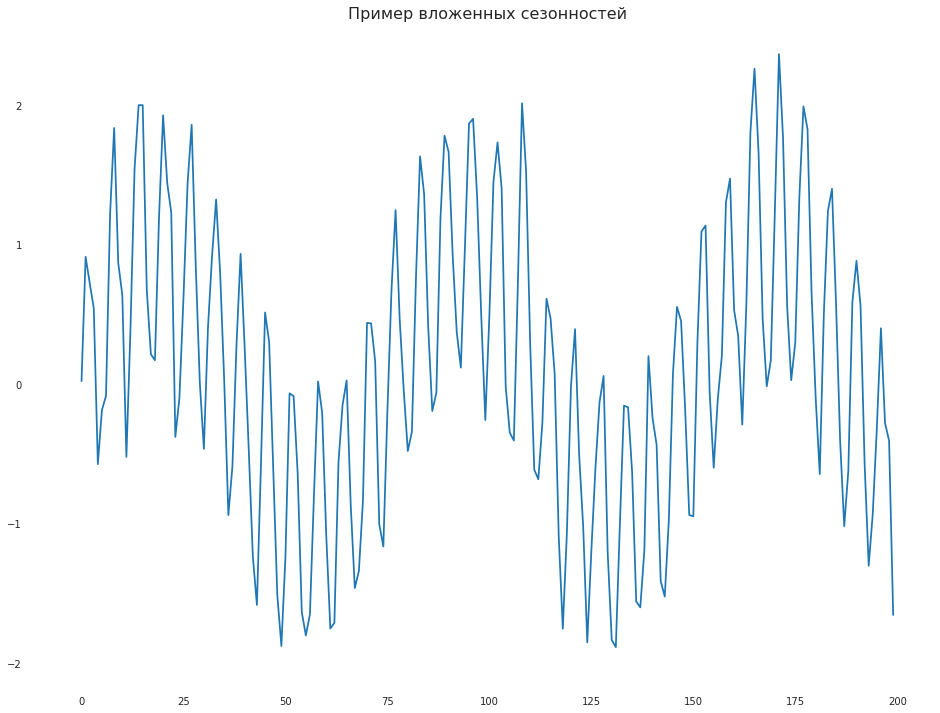
\includegraphics[width=.9\columnwidth]{img/nasted_seasonality.png}%
	\end{center}
	\caption{Пример данных со вложенной сезонностью}%
	\label{img:nasted_seasonality}%
\end{figure}

Кроме того, сезонности могут быть вложенными \ref{img:nasted_seasonality}.
Например, готовая сезонность, месячная, недельная, ежедневная.

Так же при анализе временных рядов нужно учитывать возможные выбросы.
Некоторые временные ряды могут принимать аномальные значения в праздничные дни.
Для таких случаев обычно модель проще обучить реагировать на отдельный входной
параметр, который бы характеризовал о наличии или отсутствии праздников в
определенный день.

Так как в системе может быть много параметров (и, соответственно, временных рядов),
при прогнозировании модель может вычислять будущие значения параметров разными способами:

\begin{itemize}
	\item предсказывать новые значения временного ряда на основе его прошлых значений
	\item предсказывать новые значения временного ряда на основе предыдущих значений
	нескольких параметров, которые могут повлиять на данный параметр
	\item предсказывать сразу несколько временных рядов на основании их предыдущих значений
\end{itemize}

Эти способы перечислены в порядке усложнения модели. Сложность модели влияет на
качество ее предсказаний. Однако выбор слишком сложной модели может повлечь
за собой ее переобучение. Переобучение ведет к тому, что модель теряет способность
к обобщению. Кроме того, сложные модели нужно дольше обучать. И нужно больше данных
для ее качественного обучения. Сложные модели сложнее интерпретировать.

Временные ряды, которые учитываются в модели могут быть двух типов:
эндогенные и экзогенные. Эндогенные --- это временные ряды,
которые требуется предсказать. Экзогенные ряды могут быть вычислены
наперед и не зависят от состояния исследуемой системы и эндогенных временных рядов.
Экзогенные переменные могут быть определены заранее и для прогнозируемого участка временного ряда.
Примером экзогенных переменных может служить
индикатор праздников при прогнозировании временных рядов: временной ряд этой экзогенной переменной
будет принимать значение 1 в случае, если в заданный день есть праздник и 0 в других случаях.

\textbf{Математическая модель}. Дан набор временных рядов $ A_i: a_{i,0}, a_{i,1}, ... a_{i,n} $
и набор экзогенных временных рядов $ X_j: x_{j,0}, x_{j,1}, ... x_{j,n},  x_{j,n+1}, ...  x_{j,n+h} $.
Где $h$ --- горизонт прогнозирования, количество значений временного ряда, которые требуется предсказать.
Необходимо с помощью значений $ A_i $ и $ X_j $ определить значения $ a_{i,n+1}, ... a_{i,n+h} $.

Основные виды моделей для предсказаний временных рядов \cite{voron}:
\begin{itemize}
	\item Aвторегрессионные модели --- значения временного ряда в данный момент
	линейно зависят от предыдущих значений этого же ряда
	\item Адаптивные модели --- самонастраивающиеся модели,
	которые способны отражать изменяющиеся во времени условия
	\item Нейросетевые модели
\end{itemize}

\section{Анализ методов прогнозирования временных рядов}

\textbf{Адаптивные модели} хорошо работают на большом количестве временных рядов:
в случаях, когда необходимо прогноз нужно получить быстро, а учитывать
нужно большое количество факторов. Суть адаптивных
методов заключается в том, что на каждой итерации, после того, как стали
известны новые данные, параметры модели обновляются. Параметры модели вычисляются
на основе исторических данных. Однако такие модели не могут описать сложные
зависимости.

Простота адаптивных методов компенсируется селективными и композиционными моделями.
Можно обучить несколько разных моделей и в зависимости от качества предсказаний на пошедшие
моменты времени для прогнозирования можно использовать ту модель, качество предсказаний
которой выше -~ в этом заключается идея селективных моделей. В композиционных моделях,
результирующим предсказанием выступает взвешенная сумма предсказаний моделей. Вес каждой модели
тоже адаптивный: вычисляются на основании ошибки данной модели.

Обычно адаптивные модели используются для краткосрочного моделирования.
Такие модели при прогнозировании временных рядов учитывают значения только одного временного ряда.
То, что на один временной ряд может влиять значения других временных рядов никак не учитывается.

Преимуществом адаптивных моделей можно считать их простоту и то, что они могут подстраиваться
под изменяющиеся параметры временного ряда.

Простейшим примером адаптивной модели является модель экспоненциального сглаживания:

\begin{equation}\label{eq:exp_smoothing}
	\hat{y_{t+1}} = \alpha y_t + (1 - \alpha)\hat{y_t} \\
\end{equation}

\noindent Где $ \alpha $ -~ параметр сглаживания. Наблюдения учитываются с убывающими весами.
Чем больше значение $ \alpha $, тем больше сглаживается результат вычислений модели.


\textbf{Авторегрессионные модели} могут учитывать влияние большого количества параметров
временного ряда \cite{akaike1969fitting}. Но чем больше параметров будет иметь модель, тем больше вычислений
потребуется для оценки значений этих параметров.

ARMA -~ модель авторегрессии скользящего среднего \cite{torres2005forecast}. Используется для прогнозирования
стационарных временных рядов.
ARIMA -~ это интегрированная модель авторегрессии \cite{contreras2003arima}. Позволяет объяснить тренд во временном
ряде за счет интегрирования: после того, как посчитаны разности исходного временного ряда,
пелается предположение, что эти разности -~ это стационарный ряд и предсказывается поведение
интегрированного ряда.
ARIMAX -~ модификация ARIMA \cite{peter2012arima}, в которой в модели регрессии могут учитываться не только предыдущие значения
текущего временного ряда, но и другие экзогенные переменные.
SARIMAX -~ ARIMAX с учетом сезонной компоненты \cite{omenzetter2005seasonal}. Для учета сезонной компоненты
берутся параметры авторегрессии, интегрирования и скользящего среднего с отставанием
определенным периодом сезонности.

Рассмотрим модель SARIMAX подробнее. Данная модель имеет 7 гиперпараметров:
\begin{itemize}
	\item $ p $ -~ степень авторегрессионной части модели
	\item $ d $ -~ степень интегрирования
	\item $ q $ -~ степень скользящего среднего модели
	\item $ P $ -~ степень авторегрессионной части модели для сезонной компоненты регрессии
	\item $ D $ -~ степень интегрирования для сезонной компоненты регрессии
	\item $ Q $ -~ степень скользящего среднего модели для сезонной компоненты регрессии
	\item $ S $ -~ параметр, определяющий лаг сезонности
\end{itemize}

Также отдельно стоит учитывать экзогенные переменные. Каждая переменная добавляет еще 1 коэффициент
в уравнение регрессии модели.

Определить перечисленные параметры можно перебором различных комбинаций этих параметров,
или с помощью визуального анализа.

Параметр $ d $ предназначен для того, чтобы избавиться от тренда во временном
ряде. Поэтому график дифференцирования порядка $ d $ должен выглядеть как шум.

Для определения параметра $ p $, следует изучать график частичных автокорреляций.
Если на есть статистически значимые отклонения, то индекс такого отклонения должен соответствовать
значению данного параметра.

Для определения параметра $ q $ необходимо найти статистически значимые отклонения
для автокорреляции ряда.

Важно отметить, что параметры $ p $, $ q $ должны оцениваться для дифференцированного графика.

Тогда формула для модели $ ARIMAX $:

\begin{equation}
	\bigtriangleup^{d} X_t = c + \sum_{i=1}^{p}{ a_i\bigtriangleup^{d}X_{t-i} } + \sum_{j=1}^{q}{ b_{j} \varepsilon_{t-j} + \varepsilon_t }
\end{equation}

\noindent Где $ \bigtriangleup^{d} $ --- оператор разности временного ряда. $ a_{j} $ --- авторегрессионные
коэффициенты.  $ b_{j} $ --- коэффициенты скользящего среднего. $ c $ --- константа.
Для модели с учетом сезонностей добавляются такие же слагаемые, но в них
оператор разности заменен на сезонный оператор разности.
Разности начинают вычисляться начиная не для текущего значения временного ряда,
а начиная с шага $ t - S $. Где $ t $ --- номер текущей итерации. $ S $ --- показатель лага сезонности.

В \textbf{нейросетевых моделях} тоже можно учесть влияние одного параметра системы на другие.
Суть данных методов похожа на предыдущие: сначала настраиваются начальные
значения параметров модели, а потом эти параметры обновляются, если добавляются новые данные.
Основным отличием можно считать то, что в предсказании одного временного ряда можно
учитывать значения других временных рядов в разные промежутки времени.

Нейросетевые методы можно разделить на 2 вида:
\begin{itemize}
	\item сети прямого распространения \cite{svozil1997introduction}
	\item рекуррентные \cite{zaremba2014recurrent}
\end{itemize}

Сети прямого распространения не подразумевают какого-либо состояния.
Поэтому передать информацию о предыдущем шаге итерации можно только явно:
предыдущие значения временного ряда должны передаваться на вход модели.
К сожалению, при таком подходе, количество параметров сети возрастает очень быстро
при увеличении количества предыдущих значений временного ряда. Это сильно усложняет модель,
она легко переобучается. И не может адекватно предсказать новые значения для временного ряда,
потому что теряет способность к обобщению.

Рекуррентные сети наравне с параметрами имеют внутреннее состояние , которое обновляется на каждой
итерации. Это означает, что предсказание будущих значений рядов зависит от "контекста",
то есть от предыдущих вычислений. Данные сети также могут учитывать влияние других
временных рядов на текущий даже с учетом нескольких предыдущих значений.

Но при описании влияния нескольких временных рядов в нейросетевых моделях
нельзя описать, на какой именно ряд влияет другой ряд. Такие знания могут быть у
экспертов. И потенциально, эти знания могли бы упростить модель и уменьшить количество
параметров в ней.

% http://www.machinelearning.ru/wiki/images/archive/c/cb/20160412121749!voron-ml-forecasting-slides.pdf
% деревья решений?


\section{Описание алгоритма работы нечетких когнитивных карт}

Когнитивная карта – схема причинно-следственных связей в системе.
Когнитивная карта представляет из себя ориентированный граф.
Вершины этого графа – концепты, а ребра – причинно-следственные связи между соответствующими концептами.
Когнитивные карты строятся для того, чтобы понять и проанализировать структуру сложной системы.
Каждое ребро когнитивной карты имеет свой вес, который характеризует степень влияния одного концепта на другой.

Обычно при прогнозировании с использованием нечетких когнитивных карт существует один целевой концепт,
значение которого необходимо спрогнозировать.


Стандартная формула для пересчета значений концептов нечетких когнитивных карт:

\begin{equation}\label{eq:concepts_recalc}
	A_j(t+1) = p( A_j(t) + \sum_{i = 1, i \neq j}^{n} w_{ij} A_i(t) )
\end{equation}

\noindent Где $ A_i(t) $ - значение концепта $A_i$ на шаге $t$. $ p(x) $ - функция активации:

\begin{equation}\label{eq:sigmiog_actiovation}
	p(x) = \frac {1} {1+ e^{-mx} }
\end{equation}

\noindent Параметр $ m $ определяет, на сколько сигмоида будет похожа на пороговую функцию.

В зависимости от задачи и данных, с которыми работает эксперт могут использоваться и другие
функции активации.

После того, как эксперт построил карту, он может приступить к моделированию поведения
системы и изучением причинно-следственной связи. Таким образом, эксперт может посмотреть,
как изменение одного концепта может повлиять на поведение системы в целом.

Если значения концептов карты расходятся, эксперту нужно или попробовать изменить функцию
активации или изменить значения весов концептов. Возможно, карта несбалансированна из-за
того, что в ней отсутствует еще один компонент, который вносит значительный вклад в поведение системы.

Пересчет значений концептов проходит итеративно. Имея исторические данные эксперт может
подобрать значения весов таким образом, чтобы смоделированное поведение системы как можно меньше отличалось
от экспериментальных данных. В случае классических когнитивных карт эксперту нужно это делать вручную.

После того, как эксперт оптимизировал значения весов, можно приступить к изучению причинно-следственных
связей.

Когнитивные карты можно классифицировать:

\begin{itemize}
	\item Нечеткие
	\item Нейро-нечеткие
	\item Расширенные-нечеткие
	\item Четкие
	\item Нейро-четкие
	\item Расширенные четкие
\end{itemize}

Нечеткие когнитивные карты используются для тех задач, в которых
нельзя явно оценить значения концептов. Для того, чтобы получить
численное представление нечеткого терма, используются функции фаззификации.
Обратная процедура (преобразование нечеткого числа в лингвистические переменные)
называется дефаззификацией.

Нейро-нечеткие когнитивные карты позволяют настроить веса карты
с помощью искусственных нейронных сетей. Это позволяет ускорить процесс построения карты.

В расширенных нечетких когнитивных картах появляется возможность
задавать отложенную активацию весов и более гибко формировать
связи между концептами с посмощью правил "ЕСЛИ-ТО".

Четкие когнитивные карты отличаются от нечетких тем, что
вместо нечетких чисел, в них используются четкие. Это позволяет
делать получить более точные модели.
Четкие карты являются частным случаем нечетких \cite{kayashev2014cognitive}: отличаются только отсутствием
процедур фаззицикации и дефаззификации.

Таким образом, решение использовать ли четкие числа или нечеткие
определяется прежде всего предметной областью и данными, которые
необходимо исследовать. Предпочтительным является использование
четких чисел. Но можно стоить модели, в которых бы использовались
как четкие, так и нечеткие числа, так как четкие когнитивные
карты --- это честаный случай нечетких.

\section{Интеграция нечетких когнитивных карт и нейросетей для предсказания временных рядов}

Нейро-нечеткая система - это система, которая включает в себя методы нейронных сетей и методы нечеткой логики.

Поведение объекта в сложных системах прогнозировать непросто.
Часто необходимо знать не только результат прогноза,
но и причинно-следственные связи, которыми был обусловлен данный прогноз
\cite{osoba2019dags} \cite{efficient_fcms}.
Для выявления таких причинно-следственных связей используются нечеткие когнитивные карты.
Следует отметить, что корреляция между временными ряда
Они позволяют качественно оценить влияние разных компонент системы на другие компоненты.
Однако, оригинальный алгоритм для пересчета значений концептов
не может описать сложные зависимости между отдельными компонентами.
Поэтому для того, чтобы увеличить мощность множества зависимостей, которые
может описать модель системы, можно использовать нейросетевые методы.
В таком случае когнитивная карта все еще хранит данные о причинно-следственных связях.

В нейросетевых подходах установить причинно-следственные связи сложнее.
Другие системы, например, деревья решений, наоборот, очень легко интерпретируются, легко обучаются,
но имеют более слабую способность к обобщению.

Идея нечетких когнитивных карт, предложенных Коско \cite{kosko1986fuzzy} имеет следующие преимущества:

\begin{itemize}
	\item Для проведения вычислений требуются небольшие вычислительные мощности.
	\item Простота в использовании.
	\item Можно легко добавлять и удалять концепты.
	\item Можно объединять готовые модели.
\end{itemize}

Однако есть и недостатки:

\begin{itemize}
	\item Значение концепта зависит только от значений связанных концептов карты только на предыдущей итерации.
	Невозможно определить связанные во времени концепты больше, чем на одну итерацию.
	\item Для создания карты требуется большая работа по подбору весов.
\end{itemize}

Эти недостатки можно считать существенными.
С этими недостатками можно бороться, если использовать модификации нечетких когнитивных карт,
например, TTR NFCM (Thee Term Relation Neural Fuzzy Cognitive Map) \cite{threeTermNfcm}.

В отличие от классических нечетких карт TTR NFCM позволяет
определять нелинейные функции для весов и при перерасчете значений концептов может учитывать то, как
этот концепт менялся во времени. Возможность использовать нелинейные веса достигается с помощью многослойных прецептронов.
А влияние предыдущих значений концептов определяется размером временного окна, за период которого проводится перерасчет
значений концептов.


\section{Выводы}

\begin{enumerate}
	\item Адаптивные модели хорошо работают на большом количестве временных рядов,
	но не учитывают влияние других рядов на текущий. Они хорошо предсказывают простые зависимости.
	И имеют возможность адаптироваться к новому уровню процесса.
	\item Модификации регрессионных моделей могут позволить описать значительную
	часть информации о временном ряде. Они более интерпретируемы, чем нейросетевые методы, более просты.
	\item Сети прямого распространения плохо подходят для предсказания временных рядов.
	\item Рекуррентные сети хорошо подходят для предсказания временных рядов, но
	с помощью них сложно представить знания о зависимостях между временными рядами.
	\item Четкие когнитивные карты являются частным случаем нечетких. Допустимо
	использовать как четкие, так и нечеткие числа в одной когнитивной карте.
	Тип параметров карты (четкий или нечеткий) определяется прежде всего
	из данных, с которыми работает эксперт. Нечеткость --- это способ формализовать
	лингвистические переменные.
\end{enumerate}


\section{Постановка задачи работы}

В рассмотренных методах не хватает возможности структурировать экспертные знания.
Для решения этой проблемы могут быть использованы когнитивные карты.
Кроме этого, когнитивные карт разных экспертов можно объединять. Обычно
объединенная карта представляет данные более объективно, потому что возможные
ошибки одного эксперта могут быть компенсированы знаниями другого эксперта.

Целью данной работы является создание нечеткой когнитивной карты для моделирования
социально-экономических систем с использованием и нейросетевых моделей по данным открытых источников.
Необходимо протестировать разработанную модель и сравнить с существующими решениями.

Задачи данной работы:
\begin{itemize}
	\item Разработать алгоритм для интеграции нейросетевых моделей с когнитвными картами.
	\item Спроектировать и реализовать нейро-нечеткую модель для когнитивного картирования.
	\item Предобработать и проанализировать тестовый набор данных, на котором будет обучена исследуемая модель.
	\item Протестировать полученную модель на данных открытых источников социально-экономических систем.
	\item Сравнить разработанный алгоритм нейро-нечеткого моделирования с существующими решениями.
\end{itemize}


% Программная реализация алгоритмического обеспечения для решения задачи нейро-
% нечеткого моделирования социально-экономических систем по данным открытых
% источников